%!TEX root = ../thesis.tex

%\begin{savequote}[70mm]
%	The Internet is becoming the town square for the global village of tomorrow.
%	\qauthor{Bill Gates}
%\end{savequote}


\chapter{Technologies}\label{chapter:technologies}
	
	This chapter explains more in detail the underlying technologies of this project.
	Starting from the general definition of a network and the most common architectures, to radio technologies work and then micro-controllers.
	
\section{Fundamentals of network communication}
	
	\begin{center}
		\begin{minipage}[H]{0.9\columnwidth}
			\begin{center}
				``\textit{A computer network is a structure that makes available to a data processing user at one place some data processing function or service performed at another place.}''~\cite{nla.cat-vn252493}
			\end{center}
		\end{minipage}
	\end{center}
	
	Starting from the definition of a computer network by Paul E. Green, it is easy to understand its importance in today's society.
	Smartphones, personal computers and other interconnected devices have become omnipresent in modern society, in which people need to feel connected to each other via these devices.
	% https://www.irishtimes.com/business/online-services-playing-more-important-role-in-everyday-activities-1.511857
	Not only they are used for fun, leisure and other social activities, but they allow connection to services such as online banking, government services and healthcare, that require a stable and secure connection among the systems that they use in order to provide a safe and sound experience for their users.
	All this to say, networks are everywhere underneath today's technology.
	There are no services or devices that can stand on their own without sharing data to other devices, to synchronize and provide a better user experience, to get updates from the manufacturer or simply to send a keep alive message.
	
	While this raw data is important for computers, people, the final users, process it to gain information, and this exchange of information from all around the world has brought radical changes many levels, from a cultural point of view to an economic point of view.
	The possibility of having a network of information exchange is the next step of globalization, which started with the exchange of goods among countries and now brings everyone together, allowing for a cultural exchange that lets people share and unite across the globe.
	
	This big network that is used to exchange information all around the world has a special name: Internet.
	% https://en.wikipedia.org/wiki/Right_to_Internet_access	
	% https://www.diplomacy.edu/blog/right-access-internet-countries-and-laws-proclaim-it/
	Many countries, such as Finland, Spain and Greece, have recognized the importance of this network and have given people the ''right to Internet access'', also known as the right to broadband or freedom to connect
	In these countries, service providers must be able to supply a mandatory minimum connection capability to all desiring home users in the regions of the country they serve.
	
	% http://www.redbooks.ibm.com/abstracts/gg243376.html
	It is important to note that Internet, with a capital I, is a particular set of worldwide interconnected networks \cite{gg243376}, but a common network of networks is called internetwork, shortened by internet, with a lowercase i.
	
	Such distinction began in the 1980s and has been described in RFCs \footnote{\href{https://datatracker.ietf.org/doc/html/rfc871}{RFC 871 (1982): A PERSPECTIVE ON THE ARPANET REFERENCE MODEL}}$^{,}$\footnote{\href{https://datatracker.ietf.org/doc/html/rfc872}{RFC 872 (1982): TCP-ON-A-LAN}} by computer scientists that understood how ARPANET was expanding and the its dimensions were not enough anymore to accommodate the amount of data traveling from one computer to another.
	% https://en.wikipedia.org/wiki/Commodore_64
	At that time, computers such as the IBM 5150 and the infamous Commodore 64 were starting to become more and more available, even if highly priced, not only to companies and universities, but also to consumers that brought them in their households, especially with the advent of MS-DOSs, the dominant operating system throughout the 1980s and now open source \footnote{\url{https://github.com/microsoft/MS-DOS}}.
	
	As described by IBM in one of their technical books from the time, ''it is possible to divide the Internet such as the following groups of networks''\cite{gg243376}:
	\begin{itemize}[noitemsep]
		\item Backbones: large and strategical data routes among core networks and routers that compose and connect the Internet;
		\item Regional networks that connect large facilities such as universities and colleges to each other;
		\item Commercial networks that provide to their subscribers access to the Internet;
		\item Local networks which run, for example, across a campus university;
	\end{itemize}

	% Oppure prendere mappa da https://www.globalbackbone.tisparkle.com/
	\begin{figure}
		\centering
		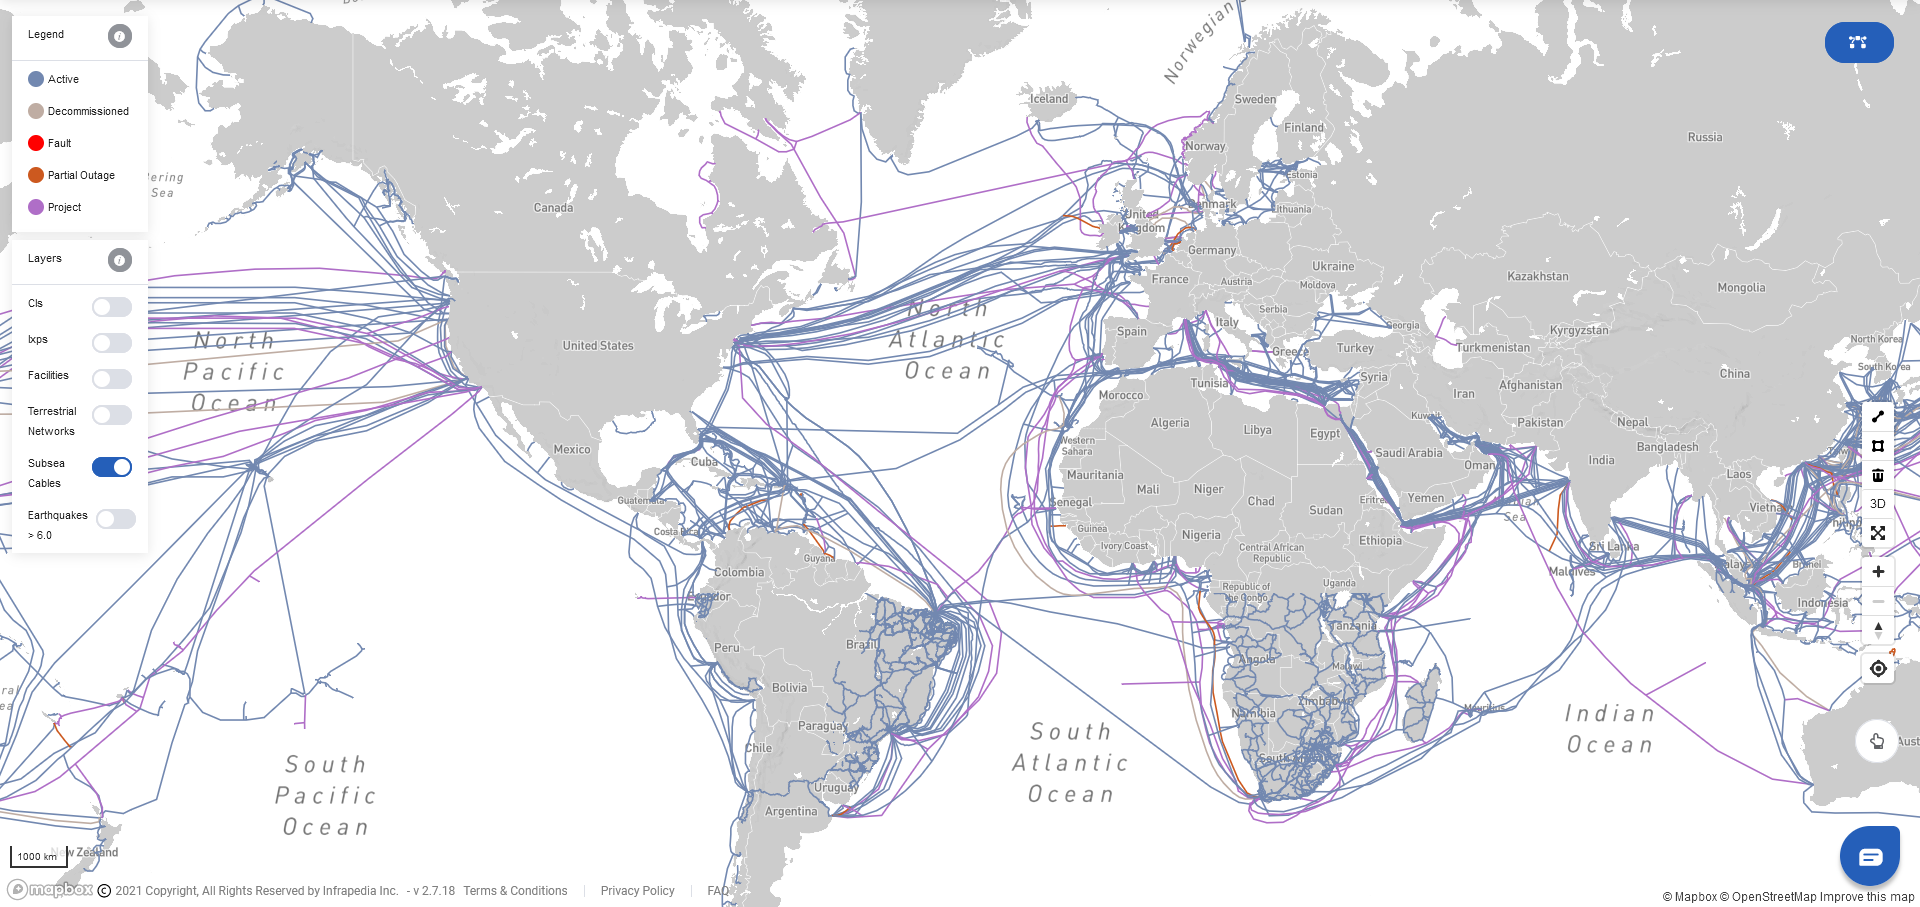
\includegraphics[width=\textwidth]{resources/img/chap3/backbone}
		\caption[Subsea Internet backbone cables between US and Europe.]{Subsea Internet backbone cables between US and Europe. \footnotemark}
	\end{figure}
	\footnotetext{\url{https://www.infrapedia.com/app}}

	Given this increase of computers connecting to the Internet, there came the need for a revised structure that could better organize these components in a more robust, but also flexible, large network.

	With the advent of Tim Berners-Lee's World Wide Web (or WWW) in 1996 and the more accessible operating systems such as windows 95 and 98, even more people bought computers
	
	So much that the dot com bubble speculated on internet related companies

	Since everyone can connect to the Internet and access it's services, there is no need for the average user to understand what happens between his machine and the rest of the network, which means he only sees the information that is displayed to him without knowing where it arrives from or what path it took to arrive on his monitor.

	
	
	% inserire immagine con la nuvoletta che si vede dentro e non si vede dentro ?
	
	% distinzione tra distributed systems e computer network
	
	\vspace{5cm}
	
	It is important to understand the difference between network architecture and network topology.
	
	A network architecture, as described by by Paul E. Green, ``is a complete definition of all the layers necessary to build the network''\cite{nla.cat-vn252493}.
	This is focused on the network software, which needs to be highly structure in order to allow for heterogeneous systems to communicate with each other.
	One example of network architecture is the ISO/OSI reference model, which is implemented by the TCP/IP stack of protocols.
	% Inserire immagine tcp/ip vs iso/osi vedi tenenbaum pag 42
	``A protocol is a set of agreements for interaction of two or more parties and is expressed by three components, syntax (e.g., a set of headers, a set of commands/responses), semantics (the actions and reactions that take place, including the exchange of messages), and timing, the sequencing and concurrency aspects of the protocol.''\cite{nla.cat-vn252493}.
	Different types of network use different architectures, based on the transmission medium and how well this performs (errors, speed, etc.)
	
	% https://www.omnisci.com/technical-glossary/network-topology
	On the other hand, the network topology refers to the manner in which the links and nodes of a network are arranged to relate to each other.
	
	% inserire immagine con le varie architetture di rete	
	
	\begin{figure}[h!]
		\centering
		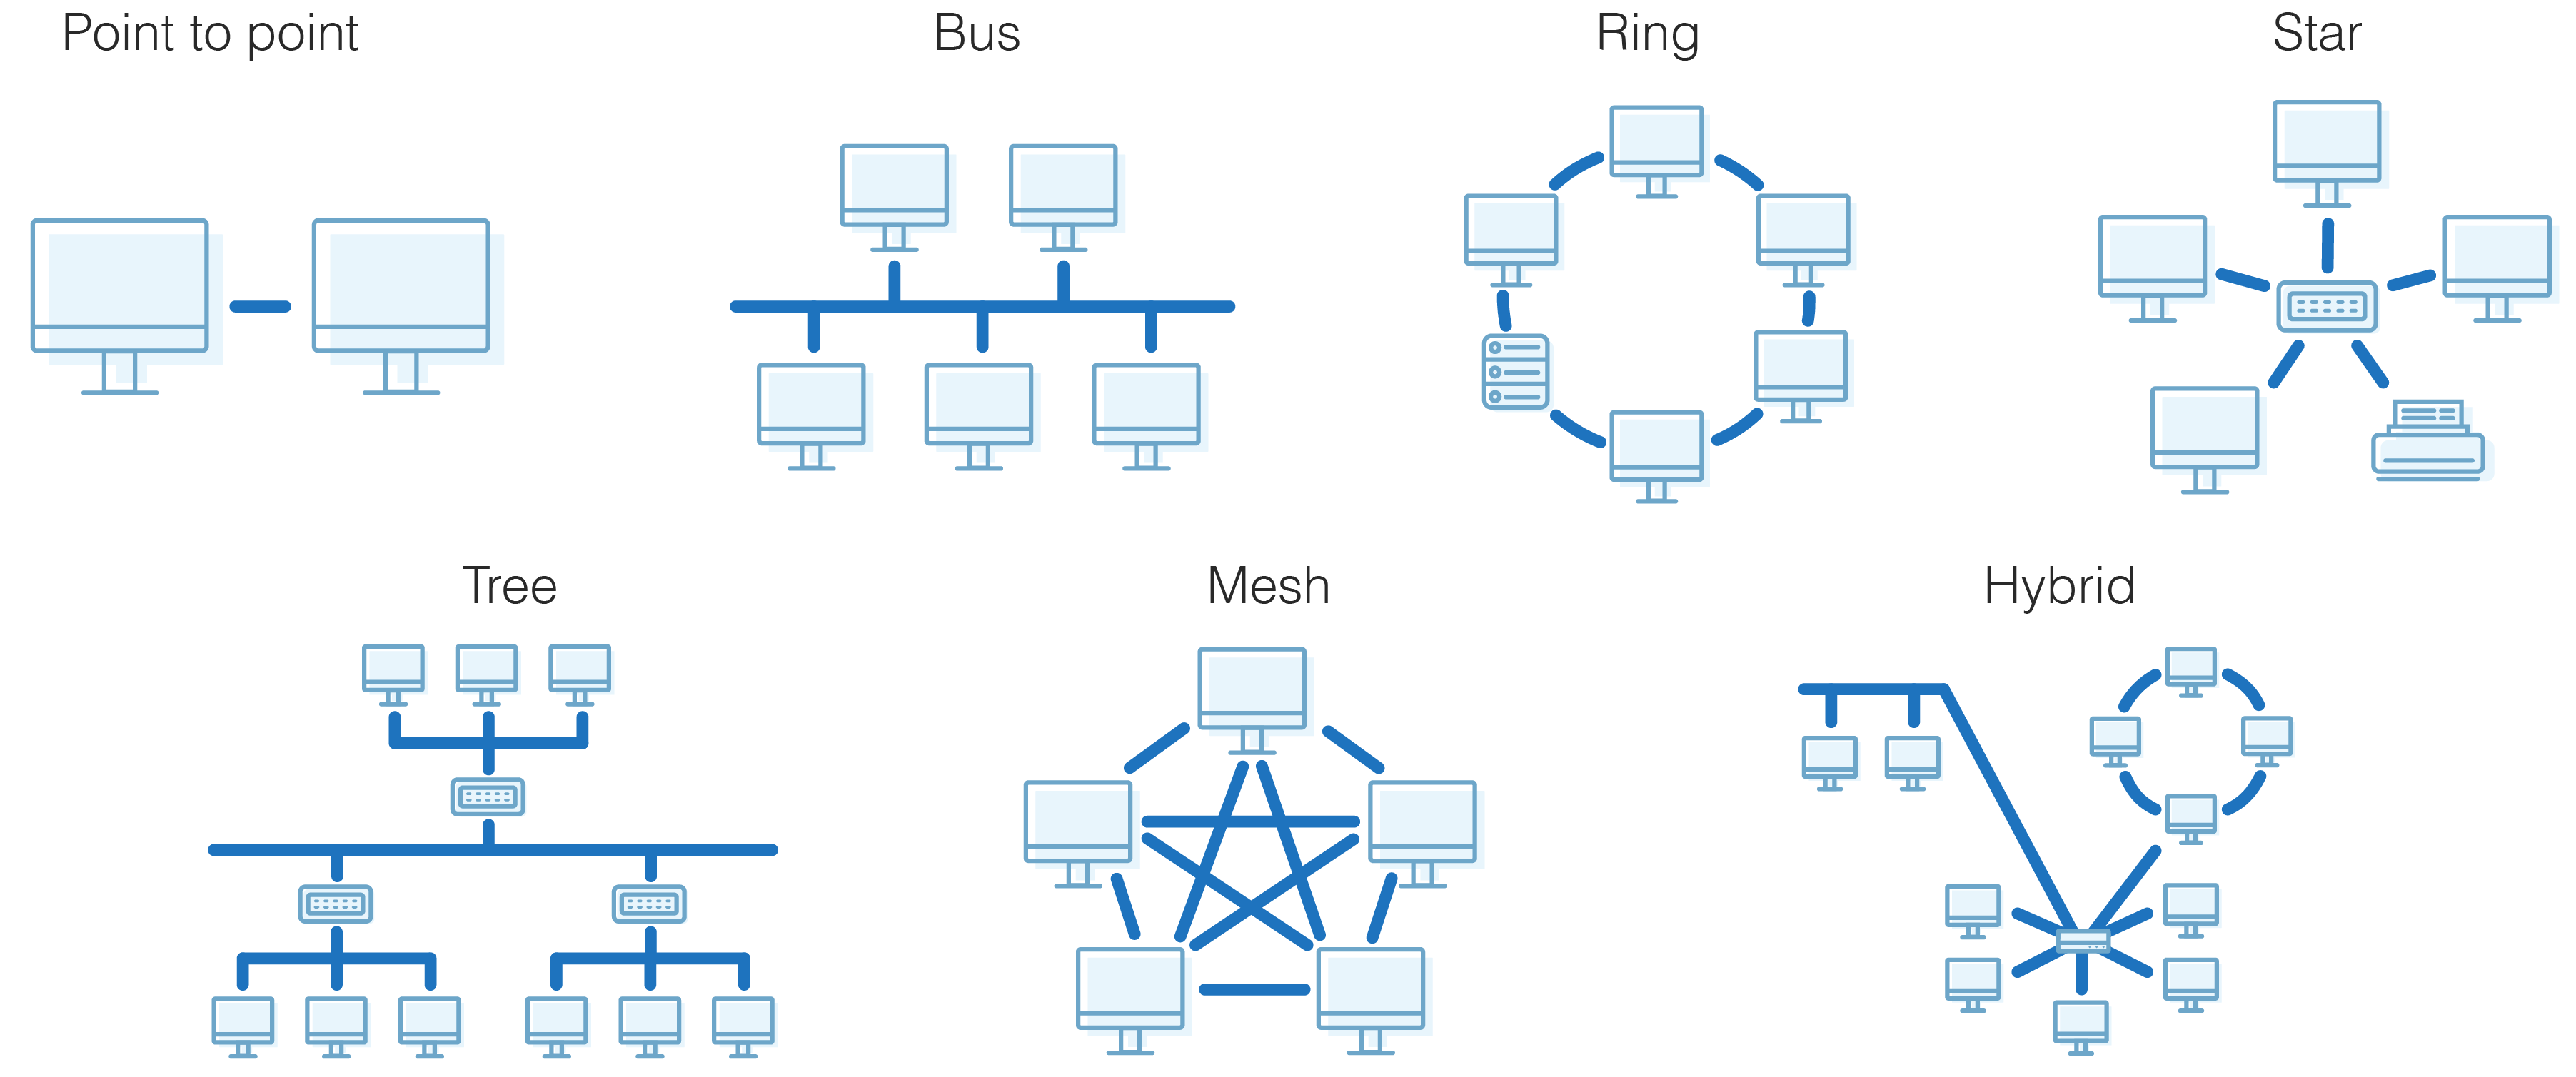
\includegraphics[width=\textwidth-4cm]{resources/img/chap3/network_topologies.png}
		\caption{Diagrammatic view of the Universal Product Code}
		\label{fig:upc_patent}
	\end{figure}
	
	dot com bubble
	
	% COPIATO DA INTERNET: responsible for technical management of IETF activities and the Internet standards process
	Nowadays, the organization responsible for technical management of IETF activities and the Internet standards process is the Internet Engineering Steering Group (IESG)\footnote{\url{https://www.ietf.org/about/groups/iesg/}}.
	It is necessary to have an organization looking over the Internet itself since it gives the regulations that allow all devices to interconnect with each other.
	
	Networks can be categorized based on their span.
	Instead, vendors apply the terms loosely to help customers distinguish among technologies.
	\begin{itemize}
		\item WAN: WAN technologies, sometimes called long haul networks, provide communication
		over long distances.
		\item MAN
		\item LAN: 	LAN technologies provide the highest speed connections among computers, but
		sacrifice the ability to span long distances.
		\item PAN
	\end{itemize}
	
	breve definizione di cloud
	
	In this thesis the mesh network that is described è contenuta nella categoria delle LAN / WAN in quanto .... 
	
	Inoltre, come verrà spiegato nel paragrafo successivo, è una rete che usa un mezzo trasmissivo radio a bassa energia, chiamata LPWAN ... 
	
	\newpage	

\section{Radio technologies}\label{sec:section_two}
	
	% TODO RIVEDERE PERCHé HAI COPIATO TROPPA ROBA DA WIKIPEDIA
	% https://en.wikipedia.org/wiki/Invention_of_radio
	Although Guglielmo Marconi is usually credited as the inventor of radio due to the creation of the first commercially successful wireless communication system, many scientists before him have studied radio waves.
	
	The idea of a wireless telegraph had been around for a while before the establishment of radio-based communication and scientist tried to achieve it via electric conduction and electromagnetic induction
	
	The discovery of electromagnetic waves, including radio waves, by Heinrich Rudolf Hertz in the 1880s came after theoretical development on the connection between electricity and magnetism that started in the early 1800s.
		
	
	
	Other important experiments were made by Nikola Tesla
	
	Tesla invented the Tesla coil during efforts to develop a "wireless" lighting system	
	Tesla employed the Tesla coil in his efforts to achieve wireless power transmission, his lifelong dream. 
	
	
	In order to give a complete picture of radio transmitting technologies, it is important to make a distinction among the ones that are made for internal or nearby use vs the ones that are used for longer distances.
	
	100 years later, radio technology has massively evolved and is used on a daily basis
	
	
	
	With new transmission technologies, new network architectures have emerged
	
	Topologies that bring computation closer to the edge are also rising, since they allow for faster computation and they bring data closer to the user
	
	LAN MAN and WAN are not enough anymore to describe the new topologies
	
	An important distinction is now made by other factors such as POWER, COST and RANGE of the transmiter receiver
	
	% TODO spiegare LPWAN
	
	Distinction of low cost vs higher cost
	% http://iotfactory.eu/iot-knowledge-center/overview-of-iot-networks/
	
	% PAPER : LPWAN Technologies: Emerging ApplicationCharacteristics, Requirements, andDesign Considerations
	\begin{figure}
		\centering
		\includegraphics[height=\textwidth, angle=90]{resources/img/iot_range}
		\caption{}
	\end{figure}
		
	% https://www.sjsu.edu/faculty/watkins/transist.htm
	da quando Tesla e Marconi studiavano questa tecnologia, l'invenzione del transistor at the infamous bell labs e la miniaturizzazione del computer, come descritto anche in [fare riferimento al paragrafo dei microcontroller], hanno permesso di implementare questi mezzi trasmissivi a vaste categorie di dispositivi 
	
	Questo ha portato alla nascita dell'Internet of Things, o IoT, come descritto anche nel Chap2.
	
	Vengono descritte adesso alcune delle più importanti tecnologie radio per il mondo dell'iot

	Altre tecnologie sono RFID, ecc. ma quelle sono per un'altra storia
	
	\subsection{LoRa}
	
		https://lora-alliance.org/
		
		https://www.semtech.com/lora
		
		\begin{figure}
			\centering
			\includegraphics[width=\textwidth]{resources/img/LoRa_Why_Range}
			\caption{}
		\end{figure}
	
	
		The smaller the package, the greater the range.
		The greater the range, the fewer receiving antennas.
		The fewer antennas, the lower the total costs for the user.

	\subsection{LoRaWAN}
	
	\subsection{Bluetooth}		
	
	\subsection{WiFi}

	IEEE 802.11, better known in the public as WiFi, short for wireless fidelity
	
	\subsection{LTE}
	

\section{LoRa and LoRaWAN}

	
	
\section{Hardware (Microcontrollers)}

	Microcontrollers (or MCUs) are compact integrated circuits designed to govern a specific operation in an embedded system.
	
	(MCU for microcontroller unit)
	
	Devices and CPUs have become smaller and more granular, allowing to have simple micro computers that need very little power resources, both computational and battery, that they can be used for very specific functions.
	
	Some examples can be:
	\begin{itemize}
		\item smog detector, which sounds an alarm when excess smog is sensed
		\item car range detector, that sends an alarm to the car's braking system when there is an object in front of it
		\item etc.
	\end{itemize}

	\begin{figure}
		\centering
		\includegraphics[width=0.75\textwidth]{resources/img/chap3/generic_board}
		\caption{}
	\end{figure}

	\subsection{Arduino}
	
		% https://www.arduino.cc/en/Main/AboutUs
		
		First commercially available microcontroller
		
		% https://www.oreilly.com/library/view/arduino-a-technical/9781491934319/ch01.html	
		
		In 2005, 
		was developed by Massimo Banzi Et Al. in Ivrea, Italy.
		
		They wanted a device that was simple, easy to connect to various things (such as relays, motors, and sensors), and easy to program. It also needed to be inexpensive, as students and artists aren’t known for having lots of spare cash. 
		
		They selected the AVR family of 8-bit microcontroller devices from Atmel and designed a self-contained circuit board with easy-to-use connections, wrote bootloader firmware for the microcontroller, and packaged it all into a simple integrated development environment (IDE) that used programs called “sketches.” The result was the Arduino.
		
		% ---
		
		The most famous version is the UNO, The UNO is the most used and documented board of the whole Arduino family.
		
		% https://www.circuito.io/blog/arduino-uno-pinout/
		This board does not provide any sensors or ports for external connectivities.
		The current revision of the board provides 
		
		Arduino Uno is based on the ATmega328 by Atmel. The Arduino Uno pinout consists of 14 digital pins, 6 analog inputs, a power jack, USB connection and ICSP header. 
		
		%--
		
		\noindent
		\begin{minipage}{0.5\textwidth}% adapt widths of minipages to your needs
			\includegraphics[width=\textwidth]{resources/img/chap3/ATMega328}
			\captionof{figure}{ company logo}
		\end{minipage}%
		\hfill%
		\begin{minipage}{0.55\textwidth}\raggedright
			Yesterday,\\
			all my troubles seemed so far away\\
			Now it looks as though they're here to stay\\
			Oh, I believe in yesterday.				Yesterday,\\
			all my troubles seemed so far away\\
			Now it looks as though they're here to stay\\
		\end{minipage}	
		
		Per quanto riguarda il linguaggio di programmazione... 
		be programmed in C and C++ programming languages using a special software called Arduino IDE
		
		Many shields that add various functionalities have been developed for this board, some examples are :  motor shield, ecc.
		
		La scelta di rendere le schematiche di arduino open source ha favorito la nascita di nuove board con capacità simili ma da produttori diversi
		Inoltre i maker sono stati in gradi di strip down to the single components when needed 
		Questa scelta è rimasta nel tempo in quanto anche per i nuovi prodotti è possibile scaricare il datasheet con le specifiche di come sono legati i componenti tra di loro
		
		Newer arduino boards offrono queste funzionalità integrate, ad esempio 
		% https://store.arduino.cc/collections/boards/products/arduino-mkr-nb-1500
		Arduino MKR NB 1500 contiene
		% https://store.arduino.cc/collections/boards/products/arduino-mkr-wifi-1010
		Arduino MKR WiFi 1010
		% https://store.arduino.cc/collections/boards/products/arduino-nano-33-ble-sense
		Arduino Nano 33 BLE Sense
				
		\begin{figure}
			\centering
			\includegraphics[width=\textwidth]{resources/img/chap3/arduino_types}
			\caption{}
		\end{figure}
				
		In particolare quest'ultimo è stato considerato per il progetto, tuttavia è stato scartato in quanto
		
		Altri microcontroller, come esp8266 che sono stati generati da arduino sono stati scartati in quanto
						
	\subsection{Raspberry Pi}
		
		The Raspberry Pi is a tiny and affordable computer that you can use to learn programming through fun, practical projects
		
		When compared to the Arduino, the Raspberry pi offers more functionalities, since it's architecture 
				
		% https://www.electronicshub.org/raspberry-pi-vs-arduino/
		Raspberry Pi and Arduino are two very popular boards among electronics DIY builders, hobbyists and even professionals. Raspberry Pi and Arduino are quite different boards. While Arduino is aimed at quick programming and circuit prototyping, Raspberry Pi acts as a learning tool for Computer Programming 
				
		The Raspberry Pi was developed by Eben Upton at the University of Cambridge in the United Kingdom with the aim of teaching and improving programming skills of students in developing countries. While Arduino is a Microcontroller based development board, the Raspberry Pi is a Microprocessor (usually an ARM Cortex A Series) based board that acts as a computer.
		
		You can connect several peripherals like a Monitor (through HDMI or AV Port), Mouse and Keyboard (through USB), connect to internet (through Ethernet or Wi-Fi), add a Camera (through the dedicated Camera Interface), just like we do to our desktop computer.
		
		Since the entire Computer (the Processor, RAM, Storage, Graphics, Connectors, etc.) is sitting on a single Printed Circuit Board, the Raspberry Pi (and other similar boards) are called as Single Board Computers or SBC.
		
		Another important thing about Raspberry Pi is, as it is a Linux based Computer, you can develop software using several Programming Languages like C, C++, Python, Java, HTML, etc.
		
		% --
		
		As the Arduino, there are different versions of raspberry pi, each one serving different scopes
		
		spiegare quali sono 
		
		% https://en.wikipedia.org/wiki/Raspberry_Pi
		\begin{figure}
			\centering
			\includegraphics[width=\textwidth]{resources/img/chap3/raspberry_types}
			\caption{}
		\end{figure}
				
		Come mai non è stato scelto raspberry pi
			
	\subsection{Pycom}
	
%		\noindent
%		\begin{minipage}{0.5\textwidth}% adapt widths of minipages to your needs
%			\includegraphics[width=\textwidth]{resources/img/pycom-logo-new-rp1}
%			\captionof{figure}{\textit{Pycom} company logo}
%		\end{minipage}%
%		\hfill%
%		\begin{minipage}{0.55\textwidth}\raggedright
%			Yesterday,\\
%			all my troubles seemed so far away\\
%			Now it looks as though they're here to stay\\
%			Oh, I believe in yesterday.				Yesterday,\\
%			all my troubles seemed so far away\\
%			Now it looks as though they're here to stay\\
%		\end{minipage}
		
		A Pycom development board has considerably more I/O than a standard Arduino, but probably comparable to an Arduino Mega. Easy to program via Python. Good example code from Pycom. Small community. Low cost. Not at all comparable to Raspberry Pi in terms of software flexibility.
		
		% https://www.reddit.com/r/IOT/comments/kx6knr/what_do_people_think_of_pycom_products/
		A complete LoRa gateway (Pygate + WiPy + IP67 box + antenna) costs around \$100, which is pretty good. So far very stable, and it was easy to configure. There's a PoE unit, but I use WiFi (at my home).

		Come mai sono state scelte le board di pycom per il progetto

		Mettere una tabella comparativa tra arduino raspberry e picom per dimostrare le capacità computazionali di ciascuno
		
% TODO ADD TO REFERENCES
% https://docs.pycom.io/gitbook/assets/lopy4-pinout.pdf
		
		A more in depth description of how the chosen technologies interact is present in chap
